\section{Lower bound for two-level expander decomposition}
\label{sec:lb}
The goal of this section is to show that repeatedly computing EDs on the inter-cluster edges necessarily incurs a dependence on the sparsity parameter. Formally, the result is the following.

\lb*
\noindent
By Yao's minimax principle, it is sufficient to give a distribution $\mathcal{G}$ over graphs with vertex set $V$ such that any deterministic streaming algorithm that computes, with probability at least $0.9$, an $(\epsilon,\phi,\ell)$-RED of $G \sim \mathcal{G}$  takes $\Omega(n/\epsilon)$ bits of space. We are not going to use the fact that the stream can be dynamic to show the lower bound, so any stream that reveals the edges of $G \sim \mathcal{G}$  in an arbitrary order serves our purposes.

We then proceed as follows. In \cref{subsec:harddistrib} we describe our hard distribution over graphs, and show a structural property of its two-level $(\epsilon,\phi)$-RED. In \cref{subsec:reductioncomm} we introduce a communication problem, $\recover$, and show a reduction to RED. Finally, in \cref{subsec:hardcomm} we give a communication lower bound for $\recover$. We combine these results into proving~\cref{th:lb} in \cref{subsec:lbproof}.


\subsection{Hard distribution}
\label{subsec:harddistrib}
The randomness of our hard distribution $\mathcal{G}$ arises from sampling Erd\H{o}s-R\'{e}nyi graphs. We recall the definition for convenience of the reader.
\begin{definition}\label{def:er}
	Let $N$ be an integer and let $p \in [0,1]$. The distribution of Erd\H{o}s-R\'{e}nyi graphs $\er(N, p)$ is the distribution over $N$-vertex graphs $H=(U,F)$ where each pair $e \in \binom{U}{2}$ is in $F$ with probability $p$ independently of other pairs.
\end{definition}
\noindent
Let $d,m$ be integers such that $3 \le d < m < n$. We now define our hard distribution $\mathcal{G}$ over $n$-vertex  graphs $G=(V, E)$, and we illustrate it in \Cref{fig:lb}.

\begin{definition}[Distributions $\mathcal{G}$ and $\mathcal{G}'$]
	\label{def:harddistr}
 We partition $V=[n]$ arbitrarily  into two sets $S$ and $T$ with $n/2$ vertices each, and further partition $S$ into $n/m$ sets $S_1,\dots,S_{n/m}$ with $m/2$ vertices each. The distribution $\mathcal{G}_{n,d,m}$ is supported over graphs $G=(V,E)$ where $E$ is defined as follows.

\begin{enumerate}
\item  For each $i~\in~[n/m]$, the induced subgraph $G[S_i]$ is sampled independently from the Erd\H{o}s-R\'{e}nyi distribution \smash{$\er({m}/{2},4d/m)$} (see Definition~\ref{def:er} above). We denote by $\mathcal{G}'_{n,d,m}$ the distribution of the subgraph $G[S]$, i.e. \smash{$\mathcal{G}'_{n,d,m}= \er({m}/{2},4d/m)^{\otimes n/m}$}.

\item The induced subgraph $G[T]$ is a {\em fixed} $d$-regular $\psi$-expander, for $\psi = \Omega(1)$ independent of $d, m, n$. 

\item We fix for convenience an arbitrary labelling $s_{i,1},\dots,s_{i,m/2}$ of the vertices in each $S_i, \, i \in [n/m]$, and we sample $K \sim \unif([m/2])$. Then, for every $i\in [n/m]$, we add $dm/2$ edges from $s_{i,K}$ to $T$ so that each $t \in T$ has $d$ incident edges in $E(S,T)$ (one way to do so is by partitioning $T$ into $n/(dm)$ subsets $T_1, \dots, T_{n/(dm)}$ with $dm/2$ vertices each and connecting $s_{i,K}$ to each vertex of $T_{\lceil i/d \rceil}$ for every $i \in [n/m]$).
\end{enumerate}
Since the parameters $n,d,m$ are fixed hereafter, we may drop the subscript from $\mathcal{G}_{n,d,m}$ and $\mathcal{G}'_{n,d,m}$ and simply denote them by $\mathcal{G}$ and $\mathcal{G}'$ respectively.
\end{definition}

\begin{figure}[h]
	\begin{minipage}[center]{\textwidth}
		\centering
		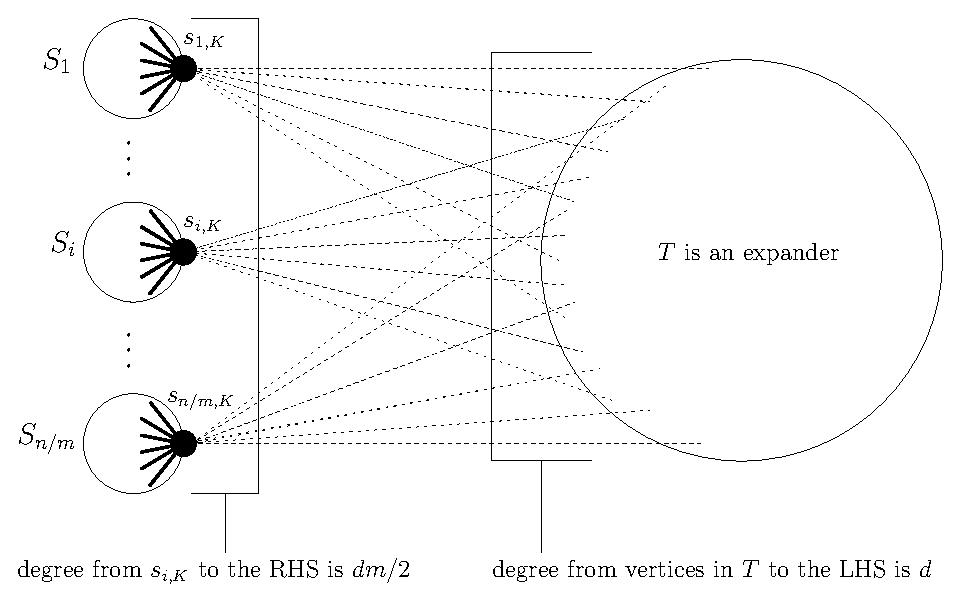
\includegraphics[scale=0.93]{lb.eps}
	\end{minipage}
	\caption{Illustration of the graph we use for proving the lower bound. Thick bullets represent important vertices, thick lines represent important edges, dotted lines represent edges connecting the important vertices to $T$.}
	\label{fig:lb}
\end{figure}

\noindent
Roughly speaking, our hard instances should be composed of $n/m$ regular expanders that are densely connected to $T$, which is also an expander, through a selection of ``special'' vertices. We will show that the hardness arises from recovering information about certain important vertices and edges, defined below and also illustrated in \Cref{fig:lb}. 



\begin{definition}[Important vertices and edges] 
	\label{def:impedges}
Let $G=(V,E) \in \supp(\mathcal{G})$. Denote by $k \in [m/2]$ the unique index such that $\{s_{i,k}:i \in [n/m]\}= \{s \in S: \{t \in T: \{s,t\} \in E\} \neq \emptyset \}$. Then, we define the set of important vertices $V^*=\{s_{i,k}:i \in [n/m]\}$ to be the set of vertices of $S$ that are adjacent to~$T$, and define the set of important edges $E^*=\{\{u, v^*\} :  u \in S\, , v^* \in V^*\}$ to be the set of edges in the induced subgraph $G[S]$ that are incident on $V^*$.
\end{definition}

\begin{remark}
	\label{rmk:harddistrib}
	Note that any sample $G \sim \mathcal{G}$ can be defined by $(G',K)$, where $G'=(S,E')$ is the graph consisting of the disjoint union of the subgraphs $(G[S_i])_{i \in [n/m]}$, and $K \in [m/2]$ is the random index determining the important vertices and edges. This is because the edges within $G[T]$ are the same for all $G \sim \mathcal{G}$, and the edges $E(S,T)$ are determined by $K$. By virtue of this observation we abuse notation and write $G=(G',K) \sim \mathcal{G}$. Moreover, for any $(G',K) \sim \mathcal{G}$ one has $G' \sim \mathcal{G}' $, and conversely, for any $G' \sim \mathcal{G}'$ and $K \sim \unif([m/2])$ one also has~$(G',K) \sim \mathcal{G}$.
\end{remark}

\noindent
In the remainder of the section, we call a graph $(1 \pm \delta)\Delta$-regular for an integer $\Delta>0$ and $\delta \in [0,1]$, if each of its vertices has degree in the range $[(1-\delta)\Delta , (1+\delta)\Delta]$. With this terminology, we show that in any valid $(\epsilon,\phi)$-ED of $G$, most of the important edges are crossing edges, as depicted in \Cref{fig:decomp}. This works under the assumption that each $G[S_i]$ is a near-regular expander.

\begin{figure}[h]
	\begin{minipage}[center]{\textwidth}
		\centering
		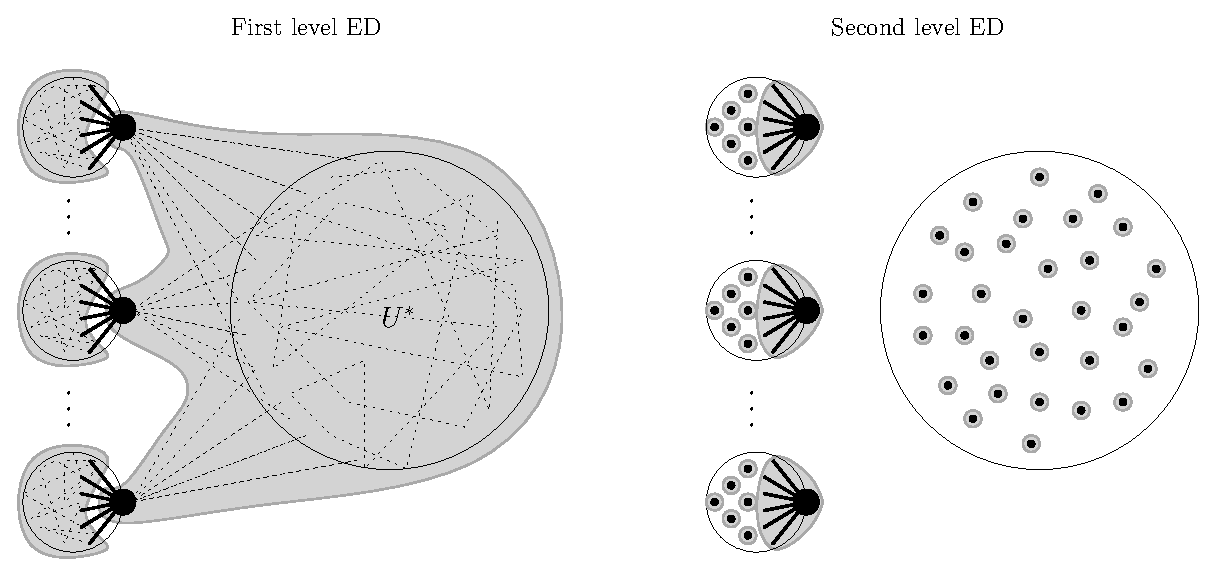
\includegraphics[scale=0.83]{lb_decomp.eps}
	\end{minipage}
	\caption{Illustration of the ideal expander decomposition of the graph. Thick bullets represent important vertices, smaller bullets represent ordinary vertices, thick lines represent important edges, dotted lines represent the rest of the edges. Grey areas represent the clusters in the decomposition.}
	\label{fig:decomp}
\end{figure}

\begin{lemma} \label{lem:special-edge}
	Let $G=(V,E) \in \supp(\mathcal{G})$, and let $\epsilon,\phi \in (0,1)$ such that $\epsilon \le 10^{-5} \cdot \psi \cdot \frac{d}{m}$ and \smash{$\phi \ge 11/m$}. If $n \ge 100 m$, $m\ge 500$, and every subgraph $(G[S_i])_{i \in [n/m]}$ is a $(1 \pm 1/10)2d$-regular $\frac{1}{3}$-expander, then any $(\epsilon,\phi)$-ED~$\mathcal{U}$ of $G$ satisfies
	\begin{equation*}
		\left| E^* \setminus \mathcal{U}\right| \ge \frac{4}{5} \cdot \left| E^*\right| \, .
	\end{equation*}
\end{lemma}

\begin{proof} 
	Let $G=(V,E) \in \supp(\mathcal{G})$ and let $k \in [m/2]$ such that the important vertices are $s_{i,k}$ for $i \in [n/m]$ (note that such value of $k$ can be uniquely inferred from seeing $G$ since the ordering of the vertices is fixed). Note that by \cref{def:harddistr} together with our assumption, the graph $G$ has at most $11/10\cdot dn/2+3/4 \cdot dn \le 1.3 dn$ edges.
	
	Hereafter, let $\mathcal{U}$ be any $(\epsilon,\phi)$-ED of $G$. We begin by arguing that there is a giant cluster in $\mathcal{U}$ that covers most of $T$ and most of the important vertices.
	
	\begin{claim}
		\label{claim:giantcluster}
		There is a component $U^* \in \mathcal{U}$ such that
		\begin{equation*}
			|T \cap U^*| \ge\left(1-12\frac{\epsilon}{\psi}\right) |T| \quad \text{and} \quad |V^* \cap U^*| \ge  \left(1-12\frac{\epsilon}{\psi}\right) |V^*| \, .
		\end{equation*}
	\end{claim}
	\begin{proof}
		For any valid $(\epsilon,\phi)$-ED $\mathcal{U}$, we must have $|E \setminus \mathcal{U}| \le \epsilon \cdot 1.3 dn$. Since $G[T]$ is a $d$-regular $\psi$-expander, there is a component $U^* \in \mathcal{U}$ that contains at least $(1-3 \epsilon/\psi) \cdot n/2$ vertices from $T$, i.e.
		\begin{equation*}
		|T \cap U^* | \ge\left(1-3\frac{\epsilon}{\psi}\right)\cdot \frac{n}{2} = \left(1-3\frac{\epsilon}{\psi}\right)|T|   \, .
		\end{equation*}
		To see why, note that if this was not the case then we could construct a cut $S = \cup_{U \in \mathcal{U}'} U \cap T$ for some $\mathcal{U}' \subseteq \mathcal{U}$ such that $3\epsilon/\psi \cdot |T| < |S| \le |T|/2$ and conclude that there would be at least $ \psi \vol_{G[T]}(S) > \epsilon \cdot 1.5 dn$ edges crossing $\mathcal{U}$.
		
		Since each vertex in $T$ has an edge to $d$ important vertices (see \cref{def:harddistr}), there are at least $(1-6\epsilon/\psi) \cdot n/m$ important vertices with at least $dm/4$ neighbours in $U^* \cap T$, i.e.
		\begin{equation*}
			\Big|\Big\{s \in V^*: \, \left|\{t \in U^* \cap T: \{s,t\} \in E\}\right| \ge \frac{1}{4}dm\Big\}\Big| \ge  \left(1-6\frac{\epsilon}{\psi}\right) \cdot \frac{n}{m} = \left(1-6\frac{\epsilon}{\psi}\right)\cdot |V^*| \, .
		\end{equation*}
		To see why, note that if this was not the case, we would have $|\{s,t\} \in E:\, s \in V^*\, , t\in T \setminus U^* \}|$ to be larger than $ (6\epsilon/\psi \cdot n/m) \cdot dm/4$, which is impossible since every $t \in T$ has $d$ incident edges in $E(S,T)$ and $|T \setminus U^*| \le 3\epsilon/\psi \cdot n/2$.
		
		Now, because most of the important vertices have many edges to $T \cap U^*$, most of these should also be in $U^*$, otherwise too many edges would cross: since $|E \setminus \mathcal{U}| \le \epsilon \cdot 1.3 dn$, there must be at most $6\epsilon/\psi \cdot n/m+\frac{\epsilon \cdot 1.3 dn}{dm/4} \le 12\epsilon/\psi \cdot n/m$ important vertices that are not in $U^*$, i.e.
		\begin{equation*}
			|V^* \cap U^*| \ge \left(1-12\frac{\epsilon}{\psi}\right) \cdot \frac{n}{m}  =  \left(1-12\frac{\epsilon}{\psi}\right) \cdot |V^*| \, .
		\end{equation*}
	\end{proof}
	\noindent
	We want to confine our attention to important vertices whose corresponding subgraph $G[S_i]$ locally preserves property~\eqref{property:crossingclassic} of \cref{def:expdecclassic}, i.e. has few inter-cluster edges as compared to its own volume. Formally, we consider the set of good vertices, defined as
	\begin{equation}
		\label{eq:defgoodvertex}
		V^*_{\text{g}} = \left\{s_{i,k} \in V^* : s_{i,k} \in U^* \, , \left|(E \setminus \mathcal{U}) \cap \binom{S_i}{2}\right| \le {200\epsilon} dm\right\} \, .
	\end{equation}
	We next show that the subgraph $G[S_i]$ corresponding to a good vertex is covered almost entirely by a single cluster, except the good vertex itself which is assigned to $U^*$.
	
	\begin{claim}
		\label{claim:separateclusters}
		Let $s_{i,k} \in V^*_{{\good}} $. Then, there is a cluster $U \in \mathcal{U}$ such that
		\begin{equation*}
			s_{i,k} \notin U \quad \text{and} \quad |U\cap S_i| \ge \left(1-700{\epsilon}\right)  |S_i| \, .
		\end{equation*}
	\end{claim}
\begin{proof}
	Since $G[S_i]$ is a $(1 \pm 1/10)2d$-regular $\frac{1}{3}$-expander by assumption, there is at least one component $U \in \mathcal{U}$ containing at least $(1-700\epsilon)m/2$ vertices in $S_i$, i.e.
	\begin{equation}
		\label{eq:badcomp}
		|U \cap S_i| \ge \left(1-700{\epsilon}\right) \frac{m}{2}  = \left(1-700{\epsilon}\right)  |S_i| \, ,
	\end{equation}
	To see why, note that if this was not the case we could construct a cut $R = \cup_{W \in \mathcal{U}'} W \cap S_i$ for some $\mathcal{U}' \subseteq \mathcal{U}$ such that \smash{$10/9 \cdot 700\epsilon \cdot |S_i| < |R| \le 9/11 \cdot  |S_i|/2$} and conclude that there would be at least $ 1/3\cdot \vol_{G[S_i]}(R) > 230\epsilon dm$ edges crossing $\mathcal{U}$ inside $S_i$, contradicting the fact that $s_{i,k} \in V^*_{{\good}} $ (see the definition in~\eqref{eq:defgoodvertex}).
	
	Hereafter, let $U \in \mathcal{U}$ be the cluster that satisfies~\eqref{eq:badcomp} (which is unique, since $\epsilon \le 10^{-5}$). We know from \cref{claim:giantcluster} that there is a cluster $U^* \in \mathcal{U}$ that contains all good vertices (by definition of good vertex, see~\eqref{eq:defgoodvertex}) and that covers most of $T$.	To show that $s_{i,k} \notin U$, we leverage the fact that $s_{i,k} \in U^*$ and that $G[U^*]$ must be a $\phi$-expander by property~\eqref{property:expanderclassic} of \cref{def:expdecclassic}. Suppose towards a contradiction that $U^* = U$, and let $Q = (U^* \cap S_i) \setminus \{s_{i,k}\}$. Because $G[S_i]$ is $(1 \pm 1/10)2d$-regular, the volume of this set in $G[U^*]$ is at least
	\begin{align*}
		\vol_{G[U^*]}(Q) & \ge -\deg_{G[S_i]}(s_{i,k}) + \sum_{u \in U^* \cap S_i} \deg_{G[U^* \cap S_i]}(u) \\
		& \ge  -\frac{11}{10}2d + \sum_{u \in U^* \cap S_i:\,\deg_{G[U^* \cap S_i]}(u) \ge (1-600{\epsilon}) \deg_{G[S_i]}(u)} \deg_{G[U^* \cap S_i]}(u) \, .
	\end{align*}
	We next observe that the sum above has at least $|U^* \cap S_i|/2$ many terms, for if this was not the case we would have at least $300\epsilon |U^* \cap S_i| \cdot 9/10 \cdot  2d \ge 200\epsilon dm$ edges from $U^* \cap S_i$ to $S_i \setminus U^*$, which would contradict $s_{i,k} \in V^*_{{\good}} $ (see the definition in~\eqref{eq:defgoodvertex}). We then continue from above and hence get
	\begin{align*}
		\vol_{G[U^*]}(Q) & \ge  -\frac{11}{10}2d + \frac{1}{2} |U^* \cap S_i|\cdot  \left(1-600{\epsilon}\right) \deg_{G[S_i]}(u)\\
		& \ge  -\frac{11}{10}2d + \frac{1}{2} |U^* \cap S_i|\cdot  \left(1-600{\epsilon}\right) \frac{9}{10} 2d\\
		\text{since $|S_i \cap U^*| \ge (1-700\epsilon) |S_i|$}\quad & \ge -\frac{11}{10}2d+\frac{9}{10}2d \frac{1}{2}\left(1-1400{\epsilon}\right) \frac{m}{2}\, .
	\end{align*}
	Moreover, we know that $|U^* \cap T| \ge (1-3\epsilon/\psi)n/2 \ge (1-1/8000)n/2$ by our assumption on $\epsilon$, so the fact that $G[T]$ is $d$-regular implies $\vol_{G[U^*]}(U^*) \ge \vol_{G[U^* \cap T]}(U^* \cap T) \ge dn/10$. Also, by near-regularity of $G$ and because $m \le n/100$, we have $\vol_{G[U^*]}(Q) \le 3d \cdot m/2 < dn/20 \le \frac{1}{2} \vol_{G[U^*]}(U^*)$. This means that $Q$ is the smaller side of the cut. On the other hand, the number of edges crossing the cut $Q$ in $G[U^*]$ is too small, since vertices in $Q$ can only connect to the rest of $U^*$ through edges incident on $s_{i,k}$, i.e.
	\begin{equation*}
		\uncut{Q}{U^*} = \deg_{G[S_i]}(s_{i,k}) \le  \frac{11}{10} 2d \, .
	\end{equation*}
	Therefore, $U_i = U^*$ implies
	\begin{equation*}
		\Phi_{G[U^*]} \le \Phi_{G[U^*]}(Q) = \frac{\uncut{Q}{U^*}}{\vol_{G[U^*]}(Q)} \le \frac{\frac{11}{10} 2d}{\frac{9}{10}d \left(1-1400{\epsilon}\right) \frac{m}{2}-\frac{11}{10}2d} \le \frac{10}{m} < \phi \, ,
	\end{equation*}
	a contradiction. Here we used that $m \ge 500$, $\phi \ge 11/m$, and $\epsilon \le 10^{-5}$.
\end{proof}
	\noindent
	By virtue of \cref{claim:separateclusters}, we have the following setting: for every good vertex $s_{i,k} \in V^*_{\text{g}}$, there is one component $U$ covering a $(1-700\epsilon)$ fraction of $S_i$ except $s_{i,k}$ itself. Therefore, many important edges incident on each good vertex are crossing edges, i.e.
	\begin{equation*}
		\{\{s,s'\} \in E^* : \, s = s_{i,k}, s' \notin U^*\} \subseteq E(U^* \cap S_i, S_i \setminus U^*) \subseteq E \setminus \mathcal{U} \quad \text{for all $s_{i,k} \in V^*_{\text{g}}$,}
	\end{equation*}
	and
	\begin{equation*}
		|U^* \cap S_i| \le  |U \setminus S_i| \le 700{\epsilon}  |S_i| = 700{\epsilon} \frac{m}{2}\quad \text{for all $s_{i,k} \in V^*_{\text{g}}$.}
	\end{equation*}
	In particular, the above conditions implies that, among the important edges incident on each good vertex, at most $700\epsilon \cdot m/2$ of them can land in the same cluster $U^*$ as the good vertex itself, i.e.
	\begin{equation}
		\label{eq:pervertexguarantee}
		|\{\{s,s'\} \in E^* : \, s = s_{i,k}, s' \notin U^*\}| \ge \frac{9}{10}2d - 700{\epsilon} \frac{m}{2}  \quad \text{for all $s_{i,k} \in V^*_{\text{g}}$.}
	\end{equation}
	If there are many good vertices, we can conclude that a lot of the important edges are crossing.
		\begin{claim}
		\label{claim:mannygood}
		One has $|V^*_{\good}| \ge  \frac{49}{50}|V^*| $.
	\end{claim}
	\begin{proof}
		Since the number of crossing edges is $|E \setminus \mathcal{U}| \le \epsilon \cdot 1.3 dn$, one has
		\begin{equation}
			\label{goodvertices:2}
			\left|\left\{s_{i,k} \in V^* : \, \left|(E \setminus \mathcal{U}) \cap \binom{S_i}{2}\right| \le {200\epsilon}dm \right\}\right| \ge \left(1-\frac{1}{100}\right)\frac{n}{m}= \left(1-\frac{1}{100}\right)|V^*| \, .
		\end{equation}
		Combining~\cref{claim:giantcluster} and~the above bound, we know $V^*_{\good}$ to be large:
		\begin{equation*}
			|V^*_{\text{g}}| \ge \left(1-12\frac{\epsilon}{\psi}-\frac{1}{100}\right) \cdot |V^*| \ge \left(1-\frac{1}{50}\right) \cdot |V^*| \, ,
		\end{equation*}
		where we use the assumption that $\epsilon \le 10^{-5} \cdot \psi \cdot \frac{d}{m}$.
	\end{proof}
\noindent
	By \cref{claim:mannygood} and the bound in~\eqref{eq:pervertexguarantee}, we can conclude the proof:
	\begin{align*}
		|E^*  \setminus \mathcal{U}| \ge \sum_{s_{i,k} \in V^*_{\text{g}}} |\{\{s,t\} \in E^* : \, s = s_{i,k}\}|   \ge   \left(\frac{9}{10} - 700{\epsilon} \frac{m}{2}\frac{1}{2d}\right)2d \cdot |V^*_{\text{g}}| \, ,
	\end{align*}
	and by \cref{claim:mannygood} we get
	\begin{align*}
	|E^*  \setminus \mathcal{U}|  \ge  \left(\frac{9}{10} - 700{\epsilon}\frac{m}{2}\frac{1}{2d}\right)2d \cdot \frac{49}{50} \cdot \frac{n}{m}  \ge \frac{4}{5} \cdot |E^*|  \, ,
	\end{align*}
	where we used $\epsilon \le 10^{-5} \psi \frac{d}{m}$ in the last inequality.
\end{proof}

\subsection{Reduction to a communication problem}
\label{subsec:reductioncomm}
We introduce the two-party one-way communication problem $\recover$, defined as follows.
\begin{definition}[Communication problem $\recover$]
	\label{def:recover}
	Let $\xi >0$  be a real parameter. In the communication problem $\recover_{\xi}$,
	Alice's input is a graph $G'=(S,E')$, and Bob's output is a set of pairs of vertices $F~\subseteq~\binom{S}{2}$ such that
	\begin{enumerate}
		\item \label{recover:fsmall} $|F| \le 6 \xi\cdot |E'| $, and
		\item \label{recover:flearns} at least a $1/10$ fraction of the pairs in $F$ are edges of $G'$, i.e. $|F \cap E'| \ge 1/10\cdot |E'|$.
	\end{enumerate}
\end{definition}
\noindent
We give a reduction from $\recover_{\epsilon m}$ to $(\epsilon, \phi,2)$-RED, in the setting where Alice's input $G'$ is an $n/2$-vertex graph drawn from $\mathcal{G}'$. We recall that \smash{$\mathcal{G}'=\mathcal{G}'_{n,d,m} = \er({m}/{2}, 4d/m)^{\otimes n/m}$} is the distribution over $n/2$-vertex graphs $G'=(S,E')$ consisting of the disjoint union of $n/m$ disjoint Erd\H{o}s-R\'{e}nyi graphs on $m/2$ vertices (see \cref{def:harddistr}). We then begin by verifying that, with high probability, an input $G' \sim \mathcal{G}'$ is a collection of $n/m$ nearly regular expanders.

\begin{lemma} \label{lem:leftexpander}
	Let $G' \sim \mathcal{G}'$. If $m\ge 500$ and $d \ge 600 \log n$ then,  with probability at least $1-1/n$, for every $i \in [n/m]$ one has that the subgraph $G'[S_i]$ is a $(1 \pm 1/10)2d$-regular $1/3$-expander
\end{lemma}

\begin{proof}
	The statement follows from the following fact about Erd\H{o}s-R\'{e}nyi graphs, whose proof is deferred to \cref{apndx:randomgraphs}.
	\begin{restatable}{fact}{erdos}
		\label{prop:er}
		Let $N \ge 10$ be an integer and $p \in [0,1]$. Then, letting $\bar{d} = p(N-1)$ one has
		\begin{equation*}
			\Pr_{H=(U,F) \sim \er(N,p)}\left[\left(\Phi_H < \frac{1}{3} \right)\text{ or } \left(\exists u \in U \text{ s.t. } \left|\deg_H(u)-\bar{d}\right|>\frac{1}{11} \bar{d}\right)\right] \le 4N \cdot \exp\left(-\frac{pN}{600}\right) \, .
		\end{equation*}
	\end{restatable}
	
	\noindent
	In our case, each subgraph $G'[S_i]$ is drawn from $\er({m}/{2}, 4d/m)$, and note that $m/2 \ge 250 \ge 10$, thus meeting the precondition of \cref{prop:er}. Hence, for any $i \in [n/m]$ \cref{prop:er} gives
	\begin{equation*}
		\Pr\left[\left(\Phi_{G'[S_i]} < \frac{1}{3}\right) \text{ or } \left(\exists u \in S_i \text{ s.t. } \left|\deg_{G'[S_i]}(u)-2d\right|>\frac{1}{10}2d\right)\right] \le 2m \cdot \exp\left(-\frac{d}{300}\right) \, ,
	\end{equation*}
	where we used $m \ge 500$ to express the degree bounds in terms of $2d$ instead of $\bar{d}$.
	Therefore, taking a union bound gives
	\begin{equation*}
		\Pr\left[\forall \, i \in [n/m]\, , \left( \Phi_{G'[S_i]} \ge \frac{1}{3} \text{ and } \forall u \in S_i\, , \left|\deg_{G'[S_i]}(u)-2d\right|\le\frac{1}{10} 2d\right)\right] \ge1- \frac{1}{n} \, ,
	\end{equation*}
	where we used $d \ge 600 \log n \ge 600 \ln n$.
\end{proof}
\noindent
By virtue of the above, most of Alice's inputs  can be embedded into a sample from $\mathcal{G}$ where a large fraction of important edges are inter-cluster edges of any ED, as per~\cref{lem:special-edge}. This will allow Alice and Bob to solve $\recover_{\epsilon m}$.

\begin{reduct}
	\label{red:recover}
	Let $\mathcal{A}$ be a deterministic streaming algorithm for computing a $2$-level $(\epsilon,\phi)$-RED of a graph given in a stream of edges. For a graph $G'=(S,E') \sim \mathcal{G}'$, we reduce $\recover_{\epsilon m}$ to computing a $2$-level $(\epsilon,\phi)$-RED as follows. Alice instantiates $\mathcal{A}$ for the vertex set $V$, and feeds her edges $E'$ and the fixed edges of $G[T]$ to $\mathcal{A}$. Then, she sends the memory state $\Pi$ of $\mathcal{A}$ to Bob. Then, Bob instantiates $m/2$ copies of $\mathcal{A}$, call them $\mathcal{A}_1, \dots, \mathcal{A}_{m/2}$, and sets the memory state of them to~$\Pi$. Next, for each $k \in [m/2]$ let $G_k = (V,E_k)$ be the graph defined by $(G',k)$, and note that Bob knows the edges between $S$ and $T$ (see \cref{def:harddistr}). Then, Bob feeds the edges $E_k(S,T)$ to~$\mathcal{A}_k$. For each $k \in [m/2]$, let $\mathcal{U}^k_1,\mathcal{U}^k_2$ be the output of $\mathcal{A}_k$. Bob finally constructs his output set $F$ as follows: for each $k \in [m/2]$, if the number of non-isolated vertices in $\mathcal{U}^k_2$ is at most $3 \epsilon d n$, add the pair $\{s,s_{i,k}\}$ to $F$ for every $i \in [n/m]$ and every $s \in S_i$ that is not an isolated vertex in $\mathcal{U}^k_2$. More formally, for a partition $\mathcal{U}$ of $V$, let $V \setminus \mathcal{U} = \{u \in V: \, \{u\} \notin \mathcal{U}\}$ be the set of non-isolated vertices in $\mathcal{U}$. With this notation, Bob outputs
	\begin{equation}
		\label{eq:boboutput}
		F = \bigcup_{k\in [m/2] : |V \setminus \mathcal{U}_2^k| \le 3\epsilon dn} F_k \, , \quad \quad \text{with } F_k=\left\{ \{s,s_{i,k}\} : i \in [n/m],\, s \in S_i \cap (V \setminus \mathcal{U}_2^k) \right\} \, .
	\end{equation} 
\end{reduct}
\noindent
We remark that if Bob learns the important edges $E^*_k$ for all $k \in [m/2]$, then he learns all of $E'$.
\begin{remark}
	\label{rmk:unionimportant}
	In the setting of~\cref{red:recover}, we have $E' = \bigcup_{k \in [m/2]} E^*_k$ and $|E'| = \frac{1}{2} \sum_{k \in [m/2]} |E^*_k|$.
\end{remark}
\noindent
As suggested by \cref{rmk:unionimportant}, it is enough to ensure that each instance $\mathcal{A}_k$ recovers the important edges of $G_k$ in order for Bob to learn the edges of $G'$. We in particular restrict ourselves to indices~$k$ for which the algorithm $\mathcal{A}_k$, the graph $G_k$, and the RED $\mathcal{U}_1^k,\mathcal{U}_2^k$ are well behaved, as defined below.

\begin{definition}
	\label{def:pk}
	In the setting of~\cref{red:recover}, for every $k \in [m/2]$ let $\mathcal{P}_k$ be the property that
	\begin{equation}
		\label{eq:propertypk}
		\text{$\mathcal{U}_1^k,\mathcal{U}_2^k$ is an $(\epsilon,\phi,2)$-RED of  $G_k$}\, ,\quad \left| E^*_k \setminus \mathcal{U}^k_1\right| \ge \frac{4}{5} \cdot \left|E^*_k\right| \, , \quad |E_k^*| \ge \frac{9}{5}\frac{dn}{m}\,, \quad |E_k|\le 1.3 dn\, .
	\end{equation}
\end{definition}
\noindent
We first show a preliminary result: if there are many $k \in [m/2]$ that satisfy $\mathcal{P}_k$, then Bob's output set contains many edges of $G'$.
\begin{lemma}
	\label{lem:almostthere}
	In the setting of~\cref{red:recover}, if $\epsilon \in (0,1)$ satisfies \smash{$\epsilon \le \frac{1}{30\sqrt{m}}$}, then
	\begin{equation*}
			|E' \cap F|  \ge \frac{49}{100} \frac{dn}{m}  |\{k\in [m/2] : \mathcal{P}_k\}| \, .
	\end{equation*}
\end{lemma}
\begin{proof}
Recall from \cref{red:recover} that $F$ is made by the union of $F_k$ over 	$k \in [m/2]$. We then first give a guarantee on the $F_k$'s individually.
	\begin{claim}
		\label{claim:pkrecover}
		Let $k \in [m/2]$ such that $\mathcal{P}_k$ holds. Then
		\begin{enumerate}
			\item \label{pk:1} $|V \setminus \mathcal{U}_2^k| \le 3 \epsilon dn$, and
			\item \label{pk:2} $|F_k  \cap (E^*_k \setminus \mathcal{U}^k_1) | \ge \frac{dn}{m}-\epsilon^2 \cdot 1.3 dn$.
		\end{enumerate}
	\end{claim}
	\begin{proof}[Proof of~\eqref{pk:1}]
		Since $\mathcal{P}_k$ is verified, $\mathcal{U}_1^k,\mathcal{U}_2^k$ is an $(\epsilon,\phi,2)$-RED of  $G_k$ (see \cref{def:pk}). By definition of RED (see \cref{def:expdecrec}), we know $|E_k \setminus \mathcal{U}^k_1| \le \epsilon |E_k|$. Moreover, one can note that the number of non-isolated vertices in $ \mathcal{U}_2^k$ is at most twice the number of edges in $E_k \setminus  \mathcal{U}_1^k$. This is because every non isolated vertex must have at least one edge incident on it in $E_k \setminus  \mathcal{U}_1^k$ (which is the input to the second level ED), as otherwise property~\eqref{property:expanderclassic} of \cref{def:expdecclassic} would be violated for any $\phi > 0 $. Thus,
		\begin{equation*}
			|V \setminus \mathcal{U}_2^k| \le 2|E_k \setminus \mathcal{U}^k_1| \le 2\epsilon |E_k|  \le 3 \epsilon dn\, ,
		\end{equation*}
		where the last inequality follows because $|E_k|\le 1.3 dn$ (see \cref{def:pk}).
	\end{proof}
	\begin{proof}[Proof of~\eqref{pk:2}]
		From part~\eqref{pk:1}, together with the assumptions that $\mathcal{U}_1^k,\mathcal{U}_2^k$ is an $(\epsilon,\phi,2)$-RED of $G_k$ and $|E_k|\le 1.3 dn$ (see \cref{def:pk}), we have
		\begin{equation*}
			\left|V \setminus \mathcal{U}^k_2 \right|   \le 3\epsilon dn\quad \text{and} \quad \left|E_k \setminus \mathcal{U}_2^k \right| = \left|\left(E_k \setminus \mathcal{U}_1^k \right) \setminus \mathcal{U}_2^k\right| \le \epsilon \left|E_k \setminus \mathcal{U}_1^k \right| \le \epsilon^2 \cdot |E_k| \le \epsilon^2 1.3 dn\, .
		\end{equation*}
		We want to argue that many of the important edges $E^*_k$ of $G_k$ are present in the set of pairs $F_k$ (see \cref{red:recover}). To do this, we make the following observation for any edge $\{s,s'\} \in E^*_k \setminus \mathcal{U}^k_1 $: if none of $s,s'$ is an isolated vertex in $\mathcal{U}_2^k$, i.e. $\{s\} \notin \mathcal{U}_2^k$ and $\{s'\} \notin \mathcal{U}_2^k$, then $\{s,s'\} \in F_k$; otherwise, if $\{s\} \in \mathcal{U}_2^k$ or $\{s'\} \in \mathcal{U}_2^k$, then $\{s,s'\} \in(E_k \setminus \mathcal{U}_1^k) \setminus \mathcal{U}_2^k$ (and this is because  $\mathcal{U}_2^k$ is an ED of the graph $(V,E_k \setminus \mathcal{U}_1^k)$ and $\{s,s'\} \in E_k \setminus \mathcal{U}_1^k$ by assumption). Therefore,
		\begin{align}
			\label{eq:boundfk}
			|F_k \cap (E^*_k \setminus \mathcal{U}^k_1)| \ge |E^*_k \setminus \mathcal{U}^k_1| - |(E_k \setminus \mathcal{U}_1^k) \setminus \mathcal{U}_2^k| \, .
		\end{align}
		To conclude the claim, we use again the property $\mathcal{P}_k$: since $\mathcal{U}_1^k,\mathcal{U}_2^k$ is an $(\epsilon,\phi,2)$-RED of  $G_k$, we have
		\begin{equation*}
			\left|(E_k \setminus \mathcal{U}_1^k) \setminus \mathcal{U}_2^k \right| \le \epsilon |E_k \setminus \mathcal{U}_1^k| \le \epsilon^2 \cdot |E_k| \, .
		\end{equation*}
		Using again $\mathcal{P}_k$, we know $| E^*_k \setminus \mathcal{U}^k_1| \ge \frac{4}{5} \cdot |E^*_k|$,  $|E_k^*| \ge \frac{9}{5}{dn}/{m}$,  and $|E_k| \le  1.3 dn$, so from~\eqref{eq:boundfk} we conclude
		\begin{equation}
			|F_k \cap (E^*_k \setminus \mathcal{U}^k_1)| \ge |E^*_k \setminus \mathcal{U}^k_1| - |(E_k \setminus \mathcal{U}_1^k) \setminus \mathcal{U}_2^k| \ge  \frac{4}{5} \cdot |E^*_k|- \epsilon^2 1.3 dn \ge \frac{dn}{m}- \epsilon^2 1.3 dn\, .
		\end{equation}
	\end{proof}
	
	\noindent
	From the definition of Bob's output $F$ (see \cref{red:recover}) and by \cref{rmk:unionimportant}, one has
	\begin{align*}
		|E' \cap F|  = \left| \left(\bigcup_{k \in [m/2]} E_k^*\right) \cap  \left(\bigcup_{k \in [m/2] : |V \setminus \mathcal{U}_2^k| \le 3\epsilon dn} F_k \right) \right|
		& \ge \left| \bigcup_{k\in [m/2] : |V \setminus \mathcal{U}_2^k| \le 3\epsilon dn}  \left( E_k^* \cap  F_k \right) \right| \\
		\text{by \cref{rmk:unionimportant}} \quad & \ge \frac{1}{2} \sum_{k\in [m/2] : |V \setminus \mathcal{U}_2^k| \le 3\epsilon dn}  \left| E_k^* \cap  F_k \right| \, ,
	\end{align*}
	and we finish using \cref{claim:pkrecover}:
	\begin{align*}
		|E' \cap F|  & \ge \frac{1}{2} \sum_{k\in [m/2] : |V \setminus \mathcal{U}_2^k| \le 3\epsilon dn}  \left| E_k^* \cap  F_k \right|  \\
		\text{by part~\eqref{pk:1} of \cref{claim:pkrecover}} \quad & \ge  \frac{1}{2} \sum_{k\in [m/2] : \mathcal{P}_k  \text{ holds}}  \left| E_k^* \cap  F_k \right| \, ,
	\end{align*}
	and then
		\begin{align*}
		|E' \cap F|  \ge  \frac{1}{2} \sum_{k\in [m/2] : \mathcal{P}_k  \text{ holds}}  \left| E_k^* \cap  F_k \right|  \ge  \frac{1}{2} \sum_{k\in [m/2] : \mathcal{P}_k \text{ holds}}  \left| (E^*_k \setminus \mathcal{U}^k_1) \cap F_k\right| \, , 
	\end{align*}
	so by part~\eqref{pk:2} of \cref{claim:pkrecover} we have
	\begin{align*}
		|E' \cap F|  \ge \frac{1}{2} \sum_{k\in [m/2] : \mathcal{P}_k  \text{ holds}} \left(\frac{dn}{m} -\epsilon^2 \cdot 1.3 dn\right)   \ge \frac{49}{100} \frac{dn}{m}  |\{k\in [m/2] : \mathcal{P}_k\}| \, ,
	\end{align*}
	where we used $\epsilon \le \frac{1}{30\sqrt{m}}$ in the last inequality.
\end{proof}
\noindent
Finally, we prove that an efficient RED algorithm gives an efficient $\recover$ protocol, using the lemma we just showed.
\begin{lemma} \label{lem:ind-recover}
	Let $\epsilon,\phi \in (0,1)$ such that \smash{$\epsilon \le \min\{ 10^{-5}\psi \frac{d}{m}, \frac{1}{30\sqrt{m}}\}$} and \smash{$\phi \ge 11/m$}. If $n \ge 100 m$, $m\ge 500$, $d \ge 600 \log n$, and there is a deterministic $L$-bit space streaming algorithm $\mathcal{A}$ that computes an $(\epsilon,\phi,2)$-RED with probability at least $9/10$ over inputs $G  \sim \mathcal{G}$, then there is a deterministic protocol that solves $\recover_{\epsilon m}$ with probability at least $3/5$ over inputs $G' \sim \mathcal{G}'$ with communication complexity at most $L$.
\end{lemma}
\begin{proof}
	The protocol is given by \cref{red:recover}.  We observe that the communication complexity bound immediately follows, since $\mathcal{A}$ has space complexity $L$ by assumption, and Alice only sends to Bob the state of the algorithm.
	
	We now focus on proving correctness of the protocol with constant probability. We do this by first proving that $F$ satisfies each of the two properties of \cref{def:recover} provided that some conditions hold, and then verify that such conditions occur with constant probability.
	
	\begin{claim}[Property~\eqref{recover:fsmall} of \cref{def:recover}]
		\label{claim:deterministic1}
		If $\left|\left\{k \in [m/2]: \, \mathcal{P}_k\right\} \right| \ge\frac{m}{3}$, then $|F| \le 6 \cdot \epsilon m |E'| $.
	\end{claim}

	\begin{claim}[Property~\eqref{recover:flearns} of \cref{def:recover}]
		\label{claim:deterministic2}
		If $\left|\left\{k \in [m/2]: \, \mathcal{P}_k\right\} \right| \ge\frac{m}{3}$, then $|F \cap E'| \ge 1/10 \cdot |E'|$.
	\end{claim}
	
	\begin{claim}
		\label{claim:manypks}
		One has $
			\Pr_{G' \sim \mathcal{G}'}\left[\left|\left\{k \in [m/2]: \, \mathcal{P}_k\right\} \right| \ge {m}/{3}\right] \ge {3}/{5}$.
	\end{claim}
	\noindent
	By \cref{claim:deterministic1} and \cref{claim:deterministic2}, the protocol given by \cref{red:recover} succeeds provided that the input $G'$ satisfies $\left|\left\{k \in [m/2]: \, \mathcal{P}_k\right\} \right| \ge\frac{m}{3}$. By \cref{claim:manypks}, the latter condition is verified with probability at least $3/5$. The lemma statement is then proven, modulo showing \cref{claim:deterministic1}, \cref{claim:deterministic1}, and \cref{claim:manypks}, which we do next.
	
		\begin{proof}[Proof of \cref{claim:deterministic1}]
		As per \cref{red:recover}, $F$ is the union of $F_k=\{ \{s,s_{i,k}\} : i \in [n/m],\, s \in S_i \cap (V \setminus \mathcal{U}_2^k) \}$ over $k$ such that $|V \setminus \mathcal{U}_2^k| \le 3\epsilon dn$. Note that $|\{ \{s,s_{i,k}\} : i \in [n/m],\, s \in S_i \cap (V \setminus \mathcal{U}_2^k) \}|$ is in fact upper-bounded by $|V \setminus \mathcal{U}_2^k|$. One then gets that $|F| \le 3\epsilon dn \frac{m}{2}$. In order to relate this bound to $|E'|$, we use our assumption: for at least $m/3$ values of $k \in [m/2]$, $|E^*_k| \ge 9/5 \cdot dn/m$. By \cref{rmk:unionimportant}, this means $|E'| \ge 1/2 \cdot m/3 \cdot (9/5 \cdot dn/m) = 3/10 \cdot dn$, so one concludes $|F| \le 6 \epsilon |E'| m$.
	\end{proof}
	
		\begin{proof}[Proof of \cref{claim:deterministic2}]
		We can use \cref{lem:almostthere}, since our bound on $\epsilon$ ensures the precondition of the lemma. We then have $|E' \cap F|  \ge \frac{49}{100} \frac{dn}{m}  |\{k\in [m/2] : \mathcal{P}_k\}| $.  Now, we conclude the claim by virtue of our assumption:
		\begin{equation*}
			|E' \cap F| \ge \frac{49}{100} \frac{dn}{m}  |\{k\in [m/2] : \mathcal{P}_k\}|  \ge \frac{m}{3} \frac{49}{100} \frac{dn}{m} \ge \frac{1}{10} |E'| \, ,
		\end{equation*}
		where in the last inequality we used that our assumption further implies $|E'| \le |E_k| \le 1.3dn$ for some $k \in [m/2]$.
	\end{proof}
	
	
	\begin{proof}[Proof of \cref{claim:manypks}]
		We recall that for $G' \sim \mathcal{G}'$ and $K \sim \unif([m/2])$ one has $(G',K) \sim \mathcal{G}$ (see \cref{rmk:harddistrib}). For~$k \in [m/2]$, we then interchangeably write $\mathcal{A}(G)$ and $\mathcal{A}(G',k)$ to refer to an execution of $\mathcal{A}$ on the graph $G$ associated with $(G',k)$. Our assumption on $\mathcal{A}$ rewrites as
		\begin{equation*}
			\Pr_{G' \sim \mathcal{G}', \, K \sim \unif([m/2])}\left[\text{$\mathcal{A}(G',K)$ fails}\right]  = \Pr_{(G',K) \sim \mathcal{G}}\left[\text{$\mathcal{A}(G',K)$ fails}\right] \le \frac{1}{10} \, .
		\end{equation*}
		Now recall \cref{red:recover}: for each $k \in [m/2]$, the result of $\mathcal{A}_k$ computed by Bob is exactly $\mathcal{A}(G',k)$, where $G'$ denotes Alice's input. Therefore, using that $G'$ and $K$ are independent and that $K$ is drawn uniformly, we get
		\begin{equation*}
			\ex_{G' \sim \mathcal{G}'} \left[ \left| \left\{k \in [m/2] : \text{ $\mathcal{A}_k$ fails }\right\}\right| \right] =\ex_{G' \sim \mathcal{G}'} \left[ \left| \left\{k \in [m/2] : \text{ $\mathcal{A}(G',k)$ fails }\right\}\right| \right] \le \frac{1}{10} \cdot \frac{m}{2} \, .
		\end{equation*}
		Hence, if we sample $G' \sim \mathcal{G}'$, only a small fraction of the values of $k$ will make $(G',k)$ a failing instance. Specifically, for any $\alpha \in [1/10, 1]$, Markov's inequality gives
		\begin{equation*}
			\Pr_{G' \sim \mathcal{G}'}\left[\left| \left\{k \in [m/2] : \text{ $\mathcal{A}(G',k)$ fails }\right\}\right| > \frac{1}{\alpha}  \frac{1}{10} \cdot\frac{m}{2}\right] \le \alpha\, .
		\end{equation*}
		In other words, at least a $1-\alpha$ fraction of the probability measure of $\mathcal{G}'$ yields a graph $G'$ such that $(G',k)$ is a succeeding instance for $\mathcal{A}$ with at least a $1-0.1/\alpha$ fraction of the possible values for $k \in [m/2]$. By \cref{lem:leftexpander} (which applies since we assume $m\ge 500$, $d \ge 600 \log n$), we also have that a $1-1/n$ fraction of the measure of $\mathcal{G}'$ yields a graph $G'$ where each component is a $(1 \pm 1/10)2d$-regular $\frac{1}{3}$-expander. This in particular implies that at least a $1-\alpha-1/n$ fraction of the probability measure of $\mathcal{G}'$ yields a graph $G'$ such that:
		\begin{itemize}
			\item for every $k \in [m/2]$, the graph $G_k=(V,E_k)$ given by $(G',k)$ has $|E_k| \le 1.3 dn$, by near-regularity and \cref{def:harddistr};
			\item for every $k \in [m/2]$, the graph $G_k=(V,E_k)$ given by $(G',k)$ has $|E^*_k| \ge \frac{9}{5} \frac{dn}{m}$, by near regularity and \cref{def:harddistr};
			\item with at least a $1-0.1/\alpha$ fraction of the possible values for $k \in [m/2]$ we have the following: $\mathcal{A}_k$ outputs an $(\epsilon,\phi,2)$-RED $\mathcal{U}^k_1,\mathcal{U}^k_2$ of the graph $G=(V,E_k)$ given by $(G',k)$. Moreover, by \cref{lem:special-edge} (which applies, since our assumptions on $n$, $m$, $\epsilon$, $\phi$ meet its preconditions) one has that $\mathcal{U}_1^k$ verifies the property
			\begin{equation*}
				\left| E^*_k \setminus \mathcal{U}^k_1\right| \ge \frac{4}{5} \cdot \left|E^*_k\right|  \, .
			\end{equation*}
		\end{itemize}
		We have then obtained that at least a $1-\alpha-1/n$ fraction of the probability measure of $\mathcal{G}'$ yields a graph $G'$ such that $\mathcal{P}_k$ holds for at least a $1-0.1/\alpha$ fraction of the possible values for $k \in [m/2]$. Setting $\alpha = 3/10$ gives the claim.
	\end{proof}
\end{proof}

\subsection{Hardness of the communication problem}
\label{subsec:hardcomm}
We show that $\recover_{\xi}$ requires linear communication in the number of edges when~$G' \sim \mathcal{G}'$ and~$\xi = \epsilon m$. Intuitively, this is because Bob is only allowed to output an $\approx \epsilon m$ factor more pairs than~$|E'|$, and for an appropriate parameter regime \smash{$\epsilon m | E'| < \frac{1}{1000} \binom{m/2}{2} \frac{n}{m} $} (where \smash{$ \binom{m/2}{2} \frac{n}{m} $} is the total number of vertex pairs in a graph consisting of $n/m$ disjoint subgraphs on $m/2$ vertices).

\begin{lemma} \label{lem:lb-recover}
	Let $\epsilon \in (0,1)$ such that $\epsilon \le {10^{-33}}/{d}$. If $m\ge 500$ and $d \ge 600 \log n$, then any deterministic protocol that solves $\recover_{\epsilon m}$ with probability at least $3/5$ over inputs $G' \sim \mathcal{G}'$ requires~$\Omega(dn)$ bits of communication.
\end{lemma}
\begin{proof}
	Let us fix hereafter $\mathcal{Q}$ to be a deterministic protocol that solves $\recover_{\epsilon m}$ with probability at least $3/5$ over inputs $G' \sim \mathcal{G}'$. We define $\I^{(1)} \subseteq \supp(\mathcal{G}')$  to be the subset of input graphs $G'=(S,E')$ in the support of $\mathcal{G}'$ such that $\mathcal{Q}$ outputs correctly on input $G'$. We also partition $\supp(\mathcal{G}')$ based on the number of edges, so for every integer $t$ we define $\I_t  \subseteq \supp(\mathcal{G}')$ to be the subset of graphs $G'=(S,E') \in \supp(\mathcal{G}')$ with~$|E'| = t$. We also let for convenience \smash{$\I^{(1)}_t =\I^{(1)}  \cap \I_t$} be the subset of correct graphs with $t$ edges. For any $G'=(S,E') \in \supp(\mathcal{G}')$, we denote by $M_{G'} \in \{0,1\}^*$ the message sent by Alice on input~\smash{$G'$} using the protocol $\mathcal{Q}$.
		
	\begin{claim}
			\label{claim:mutualunif}
			If $t$ is an integer such that $t \in [9/10 \cdot dn/2 , \, 11/10 \cdot dn/2]$ and  $|\mathcal{I}^{(1)}_{t}| \ge {1}/{2} \cdot |\mathcal{I}_t| $, then
			\begin{equation*}
				\entropy\left(M_{G'} \, \middle| \, G' \in \I_t^{(1)}\right)  \ge \frac{dn}{3} \, .
			\end{equation*}
	\end{claim}
	\begin{proof}
		For any $G' \in \mathcal{I}^{(1)}_{t}$, following the reception of  $M_{G'}$, Bob deterministically outputs at most  $6\cdot(\eps
		m)\cdot|E'| = 6 \cdot \epsilon m t$ pairs of vertices \smash{$F~\subseteq~\binom{S}{2}$}, such that at least $1/10 \cdot |E'| = t/10$ of them are actually edges of $G'$. Thus, for any~$t$ and any message \smash{$M \in \{0,1\}^{\le nm}$} (where we restrained messages to be at most $nm$-bit long without loss of generality), the number of \smash{$G'\in \mathcal{I}^{(1)}_{t}$} such that \smash{$M_{G'}=M$} is at most
		\begin{align*}
			\left| \left\{G' \in \mathcal{I}^{(1)}_{t}: \, M_{G'} = M\right\}\right| & \le \sum_{j=0.1 t}^{t} \binom{6 \cdot \epsilon m t}{j} \cdot \binom{\frac{n}{m} \binom{m/2}{2}}{t-j} \\ 
			&\le \sum_{j=0.1 t }^{t} \left(\frac{\e \cdot 6 \cdot \epsilon m t}{j} \right)^j \cdot \left(\frac{\e\cdot nm/8}{t-j}\right)^{t-j}\\
			&= \e^{t} \sum_{j=0.1t}^{t}  \left(\frac{60 \cdot \epsilon m t}{ t} \right)^j \cdot \left(\frac{ nm/8}{t}\right)^{t-j} \cdot \left(\frac{t}{t-j}\right)^{t-j} \, .
		\end{align*}
		We employ the following fact to bound the above, whose proof is deferred to \cref{apndx:ineq}.
		\begin{restatable}{fact}{math}\label{prop:math1}
			For any $0 < x \le y$, $(y/x)^x \le \e^{y/\e}$.
		\end{restatable}
		\noindent
		We apply \cref{prop:math1} to the factor $(t/t-j)^{(t-j)}$ with $x = t-j$ and $y=t$, and hence we get
		\begin{align}
			\left| \left\{G' \in\mathcal{I}^{(1)}_{t}: \, M_{G'} = M\right\}\right| & \le \e^{(1+1/\e)t} \sum_{j=0.1t}^{t}  \left(60 \epsilon m \right)^j \cdot \left(\frac{nm/8}{t}\right)^{t-j}\\
			& =  \e^{(1+1/\e)t} \left(\frac{nm}{8t}\right)^{t} \sum_{j=0.1t}^{t}  \left(60\cdot \frac{\epsilon 8t}{n} \right)^j\\
		&\le  \e^{(1+1/\e)t} \left(\frac{nm}{8t}\right)^{t}  \left( {500} \cdot \frac{\epsilon t}{n} \right)^{ t/10} t \, , \label{eq:ubcorrcond}
		\end{align}
		where in the last inequality we used the upper bounds on $\epsilon$ and $t$. On the other hand, by virtue of our assumption that $|\mathcal{I}_{t}^{(1)}| \ge {1}/{2} \cdot |\mathcal{I}_t| $, one has
		\begin{align}
			\left|\mathcal{I}^{(1)}_{t}\right| & \ge \frac{1}{2} \left|\left\{G' = (S,E') \in \supp(\mathcal{G}'): \, |E'|  = t \right\}\right|  \\
			&  \ge \frac{1}{2} \left|\left\{G' = (S,E') \in \supp(\mathcal{G}'): \, \forall \, i \in [n/m] ,\, \left|E' \cap \binom{S_i}{2}\right|  = \frac{t}{n/m} \right\}\right| \\
			& = \frac{1}{2}  \binom{\binom{m/2}{2}}{\frac{t}{n/m}}^{n/m} \ge \frac{1}{2}  \binom{\frac{m^2}{16}}{\frac{t}{n/m}}^{n/m} \ge \frac{1}{2}  \left(\frac{\frac{m^2}{16}}{\frac{t}{n/m}}\right)^{\frac{t}{n/m} \cdot n/m} =  \frac{1}{2} \left(\frac{ nm}{16t}\right)^{t}\, . \label{eq:lbcorr}
		\end{align}
		Next, we rewrite
		\begin{align*}
			\entropy\left(M_{G'} \, \middle| \,  G' \in \I_t^{(1)}\right)   & \ge \info\left(G' ; M_{G'} \, \middle| \, G' \in \I_t^{(1)}\right) \\
			&  =  \entropy\left(G' \, \middle| \, G' \in \I_t^{(1)}\right)  -  \entropy\left(G'  \, \middle| \, M_{G'},  G' \in \I_t^{(1)}\right) \, .
		\end{align*}
		Now, observing that all the graphs with same number of edges have the same probability of being sampled, one can employ the upper and lower bounds derived above:
		\begin{align*}
			 & \hphantom{=} \entropy\left(G' \, \middle| \, G' \in \I_t^{(1)}\right)  -  \entropy\left(G'  \, \middle| \,M_{G'},  { G' \in \I_t^{(1)}}\right)\\
			   & \ge  \log\left(	\left|\mathcal{I}^{(1)}_{t}\right|\right) - \log \left(\max_{M \in \{0,1\}^{\le nm}} \left| \left\{H \in \mathcal{I}^{(1)}_{t}: \, M_H = M_{G'} \right\}\right|\right) \\
			\text{by \eqref{eq:lbcorr} and \eqref{eq:ubcorrcond}} & \ge t \log\left(\frac{ \frac{1}{2} \frac{nm}{16t}}{\e^{(1+1/\e)}\cdot \frac{nm}{8t} \cdot  {(t)}^{1/t}\cdot \left( 500\cdot \frac{\epsilon t}{n} \right)^{1/10} }\right) \, .
		\end{align*}
		Then, we finish using $9/10 \cdot dn/2 \le t \le 11/10 \cdot dn/2$ and $\epsilon \le {10^{-33}}/{d}$:
		\begin{align*}
		\entropy\left(M_{G'} \, \middle| \, G' \in \I_t^{(1)}\right)   \ge t \log\left(\frac{ 1/120}{\left( 500 \cdot \frac{\epsilon 11 dn}{20n} \right)^{1/10} }\right)  \ge t \log 6 \ge \frac{9}{10} \frac{dn}{2}\ge \frac{dn}{3}\, .
		\end{align*}
	\end{proof}
	
	\begin{claim}
		\label{claim:conditionlargeprob}
		One has
		\begin{equation*}
			\Pr_{G'=(S,E') \sim \mathcal{G}'}\left[  |E'| \in \left[\frac{9}{20}dn , \, \frac{11}{20}dn\right]  \, \mathrm{ and } \, \frac{\left|\I_{|E'|}^{(1)}\right|}{\left|\I_{|E'| }\right|} \ge  \frac{1}{2}\right] \ge \frac{1}{10} \, .
		\end{equation*}
	\end{claim}
	\begin{proof}
		We begin by defining for convenience
		\begin{equation*}
			x  = \Pr_{G'=(S,E') \sim \mathcal{G}'}\left[  \frac{\left|\I_{|E'|}^{(1)}\right|}{\left|\I_{|E'| }\right|} < \frac{1}{2}\right]  \, .
		\end{equation*}
		Then, by \cref{lem:leftexpander} (which applies by our assumption on $m$ and $d$), one has
		 \begin{equation}
		 	\label{eq:unionbound}
		 		\Pr_{G'=(S,E') \sim \mathcal{G}'}\left[  |E'| \in \left[\frac{9}{20}dn , \, \frac{11}{20}dn\right]  \, \mathrm{ and } \, \frac{\left|\I_{|E'|}^{(1)}\right|}{\left|\I_{|E'| }\right|} \ge  \frac{1}{2}\right]  \ge 1-\frac{1}{n} - x\, .
		 \end{equation}
		 We are left with the task of upper-bounding the probability $x$. Letting $\T = \{0, \dots, \binom{m/2}{2} \frac{n}{m}\}$ be  the set of possible numbers of edges in $G' \sim \mathcal{G}'$, we have
		 \begin{align*}
		 	& \hphantom{=} \Pr_{G'=(S,E') \sim \mathcal{G}'}\left[\mathcal{Q} \text{ outputs correctly on input } G'\right]\\
		 	& = \Pr_{G'=(S,E') \sim \mathcal{G}'}\left[G' \in \I^{(1)}\right] \\
		 	& =\sum_{t \in \T} \Pr_{G'=(S,E') \sim \mathcal{G}'}[|E'|=t] \Pr_{G'=(S,E') \sim \mathcal{G}'}[G' \in \I^{(1)} \, | \, |E'|=t] \\
		 	& = \sum_{t \in \T}\Pr_{G'=(S,E') \sim \mathcal{G}'}[|E'|=t]  \cdot \frac{\left|\I_{t}^{(1)}\right|}{\left|\I_{t}\right|} \, ,
		\end{align*}
		where the last equality holds because all the graphs with $t$  edges have the same probability of being sampled. Hence, splitting the sum one has
		\begin{align*}
			& \hphantom{=} \Pr_{G'=(S,E') \sim \mathcal{G}'}\left[\mathcal{Q} \text{ outputs correctly on input } G'\right]\\
		 	& \le \sum_{\substack{t \in \T : \\ |\I_t^(1)| < \frac{1}{2}|\I_t^(1)| }}  \Pr_{G'=(S,E') \sim \mathcal{G}'}[|E'|=t] \cdot \frac{1}{2} + \sum_{\substack{t \in \T : \\ |\I_t^(1)| \ge \frac{1}{2}|\I_t^(1)| }} \Pr_{G'=(S,E') \sim \mathcal{G}'}[|E'|=t]\cdot 1\\
		 	& = \Pr_{G'=(S,E') \sim \mathcal{G}'}\left[  \frac{\left|\I_{|E'|}^{(1)}\right|}{\left|\I_{|E'| }\right|} < \frac{1}{2} \right] \cdot \frac{1}{2} + \Pr_{G'=(S,E') \sim \mathcal{G}'}\left[ \frac{\left|\I_{|E'|}^{(1)}\right|}{\left|\I_{|E'| }\right|} \ge \frac{1}{2}\right] \cdot 1\\
		 	& = x \cdot \frac{1}{2} + (1-x) \cdot 1 = 1-\frac{x}{2}\, .
		 \end{align*}
		 If we suppose for the sake of a contradiction that $x \ge 449/500$, then
		 \begin{equation*}
		 	\Pr_{G'=(S,E') \sim \mathcal{G}'}\left[\mathcal{Q} \text{ outputs correctly on input } G'\right] \le \frac{551}{1000} < \frac{3}{5} \, ,
		 \end{equation*}
		 which contradicts our assumption on $\mathcal{Q}$. Therefore, we plug $x < 449/500$ into~\eqref{eq:unionbound} together with the assumption $n > m \ge 500$, thus  getting the claim.
	\end{proof}
	\noindent
	Let now $\mathcal{C}$ be the event that $|E'| \in [9/10 \cdot dn/2 , \, 11/10 \cdot dn/2]$ and  \smash{$|\mathcal{I}^{(1)}_{|E'|}| \ge {1}/{2} \cdot |\mathcal{I}_{|E'|}|$}.
	The size of Alice's message on input $G'=(S,E') \sim \mathcal{G}'$ is lower bounded by
	\begin{align*}
			\entropy\left(M_{G'}\right)
			& \ge \entropy\left(M_{G'} \, \middle| \, \ind_{ \mathcal{C}}, |E'|\right)  \\
			& \ge\Pr\left[  \mathcal{C} \right]    \sum_{\substack{t \in  \left[\frac{9}{20}dn , \, \frac{11}{20}dn\right] \cap \mathbb{N}:\\ \left|\mathcal{I}^{(1)}_{t}\right| \ge {1}/{2} \cdot \left|\mathcal{I}_t\right| } } \Pr\left[|E'|=t \, \middle| \, \mathcal{C} \right] \cdot \entropy\left(M_{G'} \, \middle| \, {\mathcal{C}}, |E'|=t\right) \,,
		\end{align*}
		and because conditioning does not increase entropy we rewrite
		\begin{align*}
				\entropy\left(M_{G'}\right) & \ge\Pr\left[  \mathcal{C} \right]     \sum_{\substack{\frac{9}{20}dn \le t \le  \frac{11}{20}dn :\\ |\mathcal{I}^{(1)}_{t}| \ge {1}/{2} \cdot |\mathcal{I}_t| } }\Pr\left[|E'|=t \, \middle| \, \mathcal{C} \right] \cdot \entropy\left(M_{G'} \, \middle| \, \ind_{G' \in  \I^{(1)}} ,{\mathcal{C}}, |E'|=t\right)  \\
			& \ge\Pr\left[  \mathcal{C} \right]     \sum_{\substack{\frac{9}{20}dn \le t \le  \frac{11}{20}dn:\\ |\mathcal{I}^{(1)}_{t}| \ge {1}/{2} \cdot |\mathcal{I}_t| } }\Pr\left[|E'|=t \, \middle| \, \mathcal{C} \right] \cdot \Pr\left[G' \in  \I^{(1)} \, \middle| \,  |E'|=t\right] \cdot\entropy\left(M_{G'} \, \middle| \, { G' \in \I_t^{(1)}}\right) \, .
		\end{align*}
		Finally, we use \cref{claim:mutualunif} and  \cref{claim:conditionlargeprob} and get
		\begin{align*}
			 	\entropy\left(M_{G'}\right) & \ge \Pr\left[  \mathcal{C} \right]     \sum_{\substack{\frac{9}{20}dn \le t \le  \frac{11}{20}dn:\\ |\mathcal{I}^{(1)}_{t}| \ge {1}/{2} \cdot |\mathcal{I}_t| } } \Pr\left[|E'|=t \, \middle| \, \mathcal{C} \right] \cdot \frac{1}{2} \cdot  \frac{dn}{3}  \\
			 	& =  \frac{dn}{6} \Pr_{G'=(S,E') \sim \mathcal{G}'}\left[  |E'| \in \left[\frac{9}{20}dn , \, \frac{11}{20}dn\right]  \, \mathrm{ and } \, \frac{\left|\I_{|E'|}^{(1)}\right|}{\left|\I_{|E'| }\right|} \ge  \frac{1}{2}\right] \\
			 	& \ge  \frac{dn}{60} \, .
	\end{align*}
\end{proof}

\subsection{Proving  the lower bound}
\label{subsec:lbproof}
Finally, we set $d$ and $m$ depending on $\epsilon,\phi,n$ so as to combine \cref{lem:ind-recover} and \cref{lem:lb-recover} and conclude our streaming lower bound.
\lb*

\begin{proof}
	We recall that for any $\epsilon = 1-\Omega(1)$, computing an $(\epsilon,\phi)$-ED with constant probability requires $\Omega(n \log n)$ bits for all $\phi \in (0,\epsilon]$. To see why, consider an input graph that is a matching of size $n/10$, and notice that an ED is a $1-\epsilon$ fraction the edges. Therefore, we now consider the case $\epsilon =  O(1/\log n)$ and prove an $\Omega(n/\epsilon)$ lower bound.
	
	Let $\epsilon,\phi \in (0,1)$ be any ED parameters and define $c = \psi \cdot 10^{-40}$. Note that $c$ is a constant since $\psi = \Omega(1)$ is the fixed sparsity from \cref{def:harddistr}. In order to apply  \cref{lem:ind-recover} and \cref{lem:lb-recover}, we use distributions  $\mathcal{G}$ and $\mathcal{G}'$ from \cref{def:harddistr} with $d$ and $m$ set as follows:
	\begin{equation}
		\label{set:dm}
		d = \frac{\epsilon}{2c^3 \phi } + \frac{c}{2 \epsilon} \quad \text{and} \quad m = \frac{11}{c \phi} \, .
	\end{equation}
	We verify that these values meet the preconditions set by \cref{lem:ind-recover} and \cref{lem:lb-recover}, i.e. we show that $d$ and $m$ satisfy
	\begin{equation}
		\label{condition:dm}
		\epsilon \le \min \left\{10^{-5} \psi \frac{d}{m} , \, \frac{1}{30\sqrt{m}}, \, \frac{10^{-33}}{d}\right\}\, , \quad \phi \ge \frac{11}{m}\, , \quad 500 \le m \le \frac{n}{100}\, , \quad 600\log n \le d < m \, ,
	\end{equation}
	for all $\epsilon,\phi$ such that
	\begin{equation}
		\label{setting:epsphi}
		\epsilon \le \frac{c^2}{\log n} \, , \quad \phi \ge \frac{1}{c^2n} \, , \quad \text{and} \quad \frac{\epsilon^2}{c^4} \le \phi \le \epsilon \, .
	\end{equation}
	Substituting $d$ and $m$ as defined in~\eqref{set:dm} into~\eqref{condition:dm} we get
	\begin{equation*}
		10^{-5} \psi \frac{d}{m} = 10^{-5} \psi \left(\frac{\epsilon}{2c^3 \phi } + \frac{c}{2 \epsilon} \right) \cdot \frac{c\phi}{11} \ge 10^{-5} \psi \frac{\epsilon}{2c^2 11 } = 10^{75} \frac{\epsilon}{2\psi 11 } \ge \epsilon \, ,
	\end{equation*}
\begin{equation*}
	\frac{1}{30\sqrt{m}} = \frac{\sqrt{c}\sqrt{\phi}}{30\sqrt{11}} \ge \frac{\sqrt{c}\epsilon}{30\sqrt{11}c^2} \ge \epsilon\, ,
\end{equation*}
\begin{equation*}
	\frac{10^{-33}}{d} = 10^{-33}\frac{4c^3\epsilon\phi}{2\epsilon^2 + 2c^4\phi}=10^{-33}\frac{4c^3\epsilon}{2\epsilon^2/\phi + 2c^4} \ge 10^{-33}\frac{4c^3\epsilon}{2c^4 + 2c^4} = 10^{-33} \frac{\epsilon}{c} \ge \epsilon \, ,
\end{equation*}
\begin{equation*}
	\frac{11}{m} = c{\phi} \le \phi \, ,
\end{equation*}
\begin{equation*}
	m = \frac{11}{c \phi} \ge \frac{11}{c \epsilon}  \ge \log n \ge 500 \, ,
\end{equation*}
\begin{equation*}
	m = \frac{11}{c \phi} \le 11 c n \le \frac{n}{100}\, ,
\end{equation*}
\begin{equation*}
	d = \frac{\epsilon}{2c^3 \phi } + \frac{c}{2 \epsilon} \ge \frac{c}{2 \epsilon}  \ge \frac{\log n}{2c} \ge 600 \log n \, ,
\end{equation*}
\begin{equation*}
	d = \frac{\epsilon}{2c^3 \phi } + \frac{c}{2 \epsilon} \le \frac{\epsilon}{2c^3 \phi } + \frac{c}{2 \phi}  \le \frac{1}{2c \log n \phi } + \frac{c}{2 \phi}  < \frac{11}{c \phi} = m \, ,
\end{equation*}
so all the conditions~\eqref{condition:dm} are verified.
	
	With any $\epsilon,\phi$ as in~\eqref{setting:epsphi} and for our choice of $d,m$ as in~\eqref{condition:dm}, \cref{lem:ind-recover} gives that if there is an $L$-bit space deterministic streaming algorithm $\mathcal{A}$ that outputs an $(\epsilon,\phi,2)$-RED of $G \sim \mathcal{G}_{n,d,m}$ with probability at least $9/10$, then there is a deterministic protocol $\mathcal{Q}$ that solves $\recover_{\epsilon m}$ with probability at least $3/5$ over inputs $G' \sim \mathcal{G}'$ with communication complexity $L$. On the other hand, by \cref{lem:lb-recover} we know that, in the parameter regime of~\eqref{condition:dm}, the complexity of $\mathcal{Q}$ over $ \mathcal{G}'$ is at least $\Omega(dn)$. Hence,
	\begin{equation*}
		L = \Omega(dn)  = \Omega\left(\left(\frac{\epsilon}{\phi}+\frac{1}{\epsilon}\right) \cdot n \right) = \Omega\left(\frac{n}{\epsilon}\right)\, .
	\end{equation*}
 	By Yao's minimax principle, the theorem statement is proved with $C = c^{-4}$.
	
\end{proof}